% !TeX root = ../tg.tex

\chapter{异构数据对分割-联邦学习的影响以及优化方案}
\section{系统模型和问题背景}
我们考虑一个包含 $N$ 个客户端的集合，即 $\N=\{1,2,\ldots, N\}$，这些客户端通过分割-联邦学习协作训练一个全局神经网络模型。每个客户端 $n$ 都拥有一个数据集 $\Dnoi_n$，由于在数据收集和处理过程中可能存在标签错误和人为误差，该数据集可能包含标签噪声 \cite{lukasik2020does,ji2024fedfixer}。$\Dnoi_n$ 中的每一个数据样本 $i$ 被表示为 $(x_i,\tilde{y}_i)$，其中带有噪声的标签 $\tilde{y}_i$ 可能与真实标签 $y_i$ 不同,并且不同用户的数据标签分布并非独立同分布。

为了方便起见，我们为每个客户端 $n$ 定义一个干净的数据集 $\Dcle_n$，它与 $\Dnoi_n$ 相关联，但其中的标签噪声已被修正。$\Dcle_n$ 中的每个数据样本 $i$ 被表示为 $(x_i,y_i)$，其标签噪声已被去除。去除标签噪声的操作可以通过人工方式进行。令 $D_n=|\Dnoi_n|=|\Dcle_n|$ 表示客户端 $n$ 数据集中数据样本的数量。

在一个分割-联邦学习系统中，我们使用 $\omegab$ 来表示全局模型。该全局模型被划分为两个部分：一个 $l_{c}$ 层的客户端侧模型，记作 $\omegabc$；一个 $l_{s}$ 层的服务器侧模型，记作 $\omegabs$。特别地，客户端侧模型 $\omegabc$ 和服务器侧模型 $\omegabs$ 共同构成完整的全局模型，即 $\omegab = (\omegabc,\omegabs)$。

在分割-联邦学习系统中有两个服务器（如图~\ref{fig:sfl} 所示）：
\begin{figure}
    \centering
    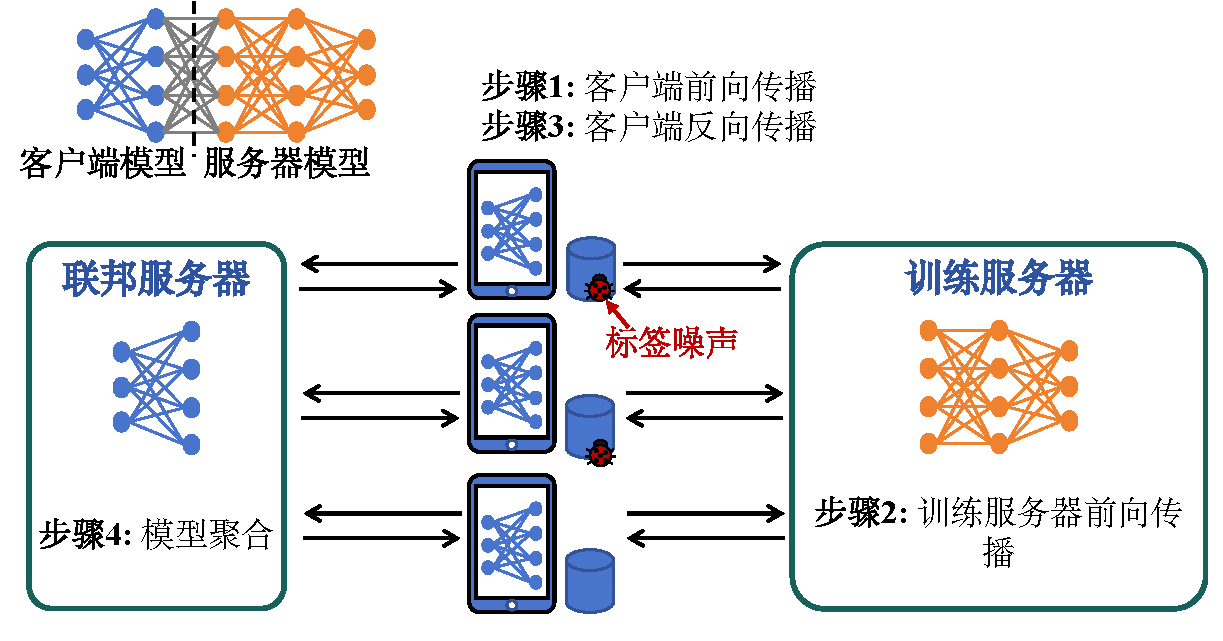
\includegraphics[height=5.6cm]{figures/sfl.pdf}
    % \vspace{-6pt}
    \caption{分割-联邦学习框架与异构数据。\vspace{-4mm}}
    \label{fig:sfl}
    % \vspace{-15pt}
\end{figure}
    
- \textbf{联邦服务器}（Fed Server），负责协调各客户端以分布式方式训练客户端侧模型 $\omegabc$；
    
- \textbf{训练服务器}（Training Server），负责以集中式方式训练服务器侧模型 $\omegabs$。


分割-联邦学习中有两种典型的算法：SFL-V1 和 SFL-V2 \cite{thapa2022splitfed}。它们的区别在于训练服务器如何更新服务器侧模型。本课题聚焦于 SFL-V2，原因如下：
\begin{enumerate}
    \item[(i)] 如文献 \cite{thapa2022splitfed} 所建议，SFL-V2 的性能通常优于 SFL-V1；
    % \item[(ii)] \rev{SFL-V1 的训练逻辑与 FedAvg 相同，只是部分训练过程被移到了服务器端进行；}
    \item[(ii)] SFL-V2 的分析比 SFL-V1 更具挑战性。\footnote{我们的分析可以通过遵循现有的联邦学习收敛性分析文献（例如 \cite{b11,karimireddy2020scaffold}）扩展到 SFL-V1。}
\end{enumerate}

\section{分割-联邦学习训练过程}\label{subsec:training}
分割-联邦学习的训练持续 $R$ 轮。在每一轮 $r$ 中，客户端 $n \in \mathcal{N}$ 从联邦服务器下载客户端侧模型 $\omegabcn^{r-1}$，该模型作为第 $r$ 轮中客户端 $n$ 的初始模型 $\omegabcn^{r}$。  
令 $\omegabs^{r}$ 表示第 $r$ 轮的服务器模型，其由上一轮的服务器模型初始化而来。在第 $r$ 轮中，客户端 $n$ 和服务器使用数据集 $\mathcal{D}_{n}^{\text{oi}}$ 对模型进行 $E$ 轮（epoch）的训练。在每一轮中，客户端将其数据集划分为多个小批量（mini-batch），并依次用于对模型 $\omegabcn^{r}$ 和 $\omegabs^r$ 进行更新。第 $r$ 轮中针对一个小批量 $\zetanoi_n \subset \mathcal{D}_{n}^{\text{oi}}$ 的训练过程包含以下四个步骤：

\textbf{步骤 1：客户端前向传播}。客户端 $n$ 使用小批量 $\zetanoi_n$ 在其本地客户端侧模型 $\omegabcn^{r}$ 上进行前向传播。

随后，每个客户端将其计算得到的中间激活值（即 $\omegabcn^{r}$ 前向传播的输出）以及数据标签发送给训练服务器。

\textbf{步骤 2：训练服务器前向传播}。训练服务器在接收到客户端的中间激活值后，在模型 $\omegabs^{r}$ 上执行前向传播以生成预测标签并计算损失函数。需要注意的是，服务器侧模型 $\omegabs^{r}$ 对某个客户端激活值的更新仅在其之前对其他更早到达的客户端激活值的更新完成后才开始。

\textbf{步骤 3：训练服务器反向传播}。训练服务器根据计算出的损失函数计算梯度，并据此更新模型 $\omegabs^{r}$。由于服务器侧模型 $\omegabs^{r}$ 仅包含完整模型中的 $l_s$ 层，训练服务器会将中间梯度发送回客户端 $n$，以便其更新客户端侧模型 $\omegabcn$。

\textbf{步骤 4：客户端反向传播}。客户端 $n$ 在接收到中间梯度后，继续完成反向传播过程，从而更新本地的客户端侧模型 $\omegabcn^r$。至此，一个小批量的训练过程完成。

\textbf{步骤 5：模型聚合}。  
在每一轮训练中，每个客户端 $n$ 需要与训练服务器进行 $E \times \left\lceil \frac{|\mathcal{D}_n|}{|\zeta_n|} \right\rceil$ 次交互，以确保客户端 $n$ 的数据被使用 $E$ 次。当所有客户端完成训练后，联邦服务器通过加权平均的方式计算全局客户端侧模型 $\omegabc^r$：
\begin{equation}\label{eq:c-agg}
\omegabc^r=\sum_{n=1}^{N}\frac{|\mathcal{D}_n|}{\sum_{n'=1}^{N}|\mathcal{D}_{n'}|}\omegabcn^r.
\end{equation}
注意，训练服务器维护着全局的服务器侧模型 $\omegabs^r$，无需对其进行聚合操作。  
当客户端和服务器完成 $R$ 轮训练后，最终的完整模型为 $\omegab^R=(\omegabc^R,\omegabs^R)$。

\section{分割-联邦学习的收敛性分析}
本部分从理论上分析带标签噪声的非独立同分布数据集对分割-联邦学习收敛性的影响 ，其中关键挑战在于回答如何在收敛性分析中量化标签噪声这一问题。



如前所述，文献\cite{ke2023impact} 在联邦学习（FL）中量化了标签噪声，但其重点是模型的泛化能力，而非收敛性，因此其分析方法在此并不适用。同时，据我们所知，目前尚无研究在分割-联邦学习或联邦学习的收敛性分析中对标签噪声进行过量化。

为填补这一空白，我们提出首先量化标签噪声对随机梯度的值及其方差 的影响，从而可以沿用传统的证明路径来推导出收敛速率。这种方法为将标签噪声纳入分割-联邦学习收敛性分析提供了分析框架，并可扩展至其他分割-联邦学习或联邦学习算法。

具体而言，令 $\zetacle_n$ 表示客户端 $n$ 的干净数据集 $\Dcle_n$ 中的一个小批量。设 $F_n(\omegab;\zetacle_n)$ 表示完整模型 $\omegab$ 在客户端 $n$ 的小批量 $\zetacle_n$ 上的损失函数。客户端 $n$ 的期望损失为  
\begin{equation}\label{eq:exp-fn}
\fcle_n\left(\omegab\right)=\mathbb{E}_{\zetacle_n\sim \Dcle_n}\left[F_n\left(\omegab;\zetacle_n\right)\right].
\end{equation}

分割-联邦学习的目标是学习一个模型 $\omegab^*$，使其最小化所有客户端上损失函数 $F_{n}(\omegab)$ 的加权平均值 \cite{b8}：
\begin{equation}\label{Objective of SFL}
\omegab^* =\arg \min_{\omegab}f(\omegab)\triangleq \sum_{n=1}^{N}\frac{|\D_n|}{\sum_{n'=1}^{N}|\D_{n'}|}F^{cle}_{n}(\omegab).
\end{equation}

需要注意的是，分割-联邦学习的训练过程是基于所有客户端 $n\in\N$ 的带噪声数据集 $\Dnoi_n$ 进行的；而如式 (\ref{Objective of SFL}) 所述，其优化目标仍然是使模型 $\omegab^R$ 拟合所有客户端的干净数据集 $\Dcle_n$。

接下来，我们将分别在标签噪声环境下，针对均方误差（MSE）损失函数与交叉熵（Cross-Entropy）损失函数对分割-联邦学习的收敛性进行分析。

\subsection{均方误差损失函数}\label{subsec:mse}
\subsubsection{标签噪声下的损失函数}
在本节中，我们考虑使用均方误差（MSE）作为损失函数。均方误差可用于机器学习中的任务，例如回归。对于这些任务，由于标签通常是连续值，我们在标签 $y_i$ 上添加一个服从正态分布的随机噪声 $\epsilon_i$，即 $\epsilon_i \sim \mathbb{N}(\mu, \sigma^2)$，其中 $\mu$ 和 $\sigma^2$ 分别为噪声的均值和方差。这种噪声设置被现有研究广泛采用（例如 \cite{frenay2013classification}）。

同时，我们设置 $\mu=0$ 以确保加入噪声后标签的平均值不变。  
则数据集 $\Dnoi_n$ 中的样本 $i$ 表示为 $(x_i,\tilde{y}_i \triangleq y_i+\epsilon_i)$。令 $h(x_i;\omegab)$ 表示使用模型 $\omegab$ 对特征 $x_i$ 的预测标签值。模型 $\omegab$ 在一个小批量 $\zeta$ 上的 MSE 损失函数 $F_{n}(\omegab;\zeta)$ 定义如下：
\begin{equation}\label{eq:mse}
F_n\left(\omegab;\zeta\right)=\frac{1}{|\zeta|}\sum_{\left(x_i,{y}_i\right)\in \zeta}\left(h\left(x_i;\omegab\right)-{y}_i\right)^2.
\end{equation}

因此，我们可以将含噪声数据集下的损失函数用干净数据集下的损失函数表示如下：

\begin{lemma}[带标签噪声的均方误差]\label{lem:mse}
考虑一个小批量 $\zetanoi_n$ 及其对应的干净小批量 $\zetacle_n$，则有
\begin{multline}
F_n\left(\omegab;\zetanoi_n\right)=F_n\left(\omegab;\zetacle_n\right)\\
    +\frac{1}{|\zetanoi_n|}\sum_{\left(x_i,\tilde{y}_i\right)\in \zetanoi_n}\left( \epsilon_i^2 - 2\left(h\left(x_i;\omegab\right)-y_i\right)\epsilon_i \right).
\end{multline}
\end{lemma}

\subsubsection{假设条件}
如同许多已有工作（例如 \cite{b4,b11,b8}），我们在收敛分析中对随机梯度和损失函数做出一些假设。令 $\gb_n\left(\omegab,\zeta_n\right)$ 表示 $F_n\left(\omegab;\zeta_n\right)$ 在小批量 $\zeta_n$ 上的随机梯度，即 $\gb_n\left(\omegab,\zeta_n\right)\triangleq \nabla F_n\left(\omegab;\zeta_n\right)$。令 $\nabla \fcle_n(\omegab)$ 表示客户端 $n\in\N$ 的干净数据集上期望损失 $\fcle_n(\omegab)$ 的梯度，定义见公式 \eqref{eq:exp-fn}。令 $\nabla \fnoi_n(\omegab)$ 表示对应于噪声数据集的期望损失梯度。对于任意客户端 $n\in\N$，来自干净数据集 $\Dcle_n$ 的小批量上的随机梯度满足以下假设：

\begin{assumption}[均方误差下随机梯度的方差]\label{ass:gradient-variance}
对于任意客户端 $n\in\N$，$\gb_n\left(\omegab,\zetacle_n\right)$ 在干净小批量上的期望方差是有界的，即：
\begin{equation}\label{eq:gradient-variance}
    \mathbb{E}_{\zetacle_n\sim \Dcle_n}\left[\left\Vert \gb_n\left(\omegab,\zetacle_n\right) - \nabla \fcle_n\left(\omegab\right) \right\Vert^2 \right] \leq \phi_n^2.
\end{equation}
\end{assumption}

\begin{assumption}[均方误差下的随机梯度]\label{ass:gradient}
对于任意客户端 $n\in\N$，$\gb_n\left(\omegab,\zetacle_n\right)$ 在 clean 数据集 $\Dcle_n$ 上的期望随机梯度是有界的，即：
\begin{equation}\label{eq:gradient}
\mathbb{E}_{\zetacle_n\sim \mathcal{D}_n^{cle}}\left[\left\Vert \gb_n\left(\omegab, \zetacle_n\right) \right\Vert^2\right] \leq G_n^2.
\end{equation}
\end{assumption}

\begin{assumption}[数据异构性]\label{ass:heter}
所有客户端 $n\in\N$ 的期望梯度 $\nabla \f_n(\boldsymbol{\omega})$ 的方差是有界的，即：
\begin{equation}
\textstyle \left\Vert 
\nabla \f_n\left(\boldsymbol{\omega}\right)- \sum_{n\in\N}
\nabla\f_n(\boldsymbol{\omega})/N \right\Vert^2 \le \lambda^2.
\end{equation}
这里，$\nabla \f_n(\boldsymbol{\omega})$ 同时表示 $\nabla \f_n^{cle}(\boldsymbol{\omega})$ 和 $\nabla \f_n^{noi}(\boldsymbol{\omega})$。\footnote{注意，非独立同分布（non-IID）和标签噪声可以建模为相互独立的事件，前者涉及客户端的数据分布，后者涉及标签如何被破坏。}

\end{assumption}

我们对损失函数作出如下假设：\footnote{虽然我们使用均方差作为损失函数，但损失函数相对于全局模型的性质依赖于分割-联邦学习中的模型结构和小批量中的数据样本。因此，如同现有工作（例如 \cite{b4,b11,b8}），我们需要对损失函数施加假设以便进行分析。}

\begin{assumption}[$S$-平滑性]\label{ass:smooth}
对于任意模型 $\omegab_1, \omegab_2\in \mathbb{R}^d$，损失函数是 $S$-平滑的，即：
$$
F_n(\omegab_2) \leq F_n(\omegab_1)+\langle \nabla F_n(\omegab_1), \omegab_2-\omegab_1\rangle +\frac{S}{2}\|\omegab_2-\omegab_1\|^2.
$$
\end{assumption}

\subsubsection{收敛性分析}\label{proofC}
我们首先分析在噪声数据集下随机梯度相关的界，然后对分割-联邦学习的收敛性进行界定。

\textbf{标签噪声存在时的随机梯度：} 考虑到数据集中存在标签噪声，\eqref{eq:gradient-variance} 和 \eqref{eq:gradient} 中定义的随机梯度 $\gb_n(\cdot)$ 相关的界会增加。特别地，含噪声数据集上的随机梯度 $\gb_n(\omegab,\zetanoi_n)$ 可表示为干净数据集上的随机梯度 $\gb_n(\omegab,\zetacle_n)$ 的表达式，如下所示：
\begin{multline}\label{Gradient of clean loss}
\gb_n\left(\omegab,\zetanoi_n\right) %= \nabla F_n\left(\boldsymbol{\omega};\zetanoi_n\right)\\
=\gb_n\left(\omegab,\zetacle_n\right)\\
-\frac{1}{|\zetanoi_n|}\sum_{\left(x_i,y_i+\epsilon_i\right)\in \zetanoi_n}2\epsilon_i \nabla h\left(x_i;\boldsymbol{\omega}\right).
\end{multline}

因此，我们可以分别界定含噪声数据集下的随机梯度的方差和值。

\begin{proposition}[均方差损失下含标签噪声的随机梯度的方差]\label{prop:variance-g mse}
在假设 \ref{ass:gradient-variance} 下，任意客户端 $n\in\N$ 在噪声小批量上的 $\gb_n\left(\omegab,\zetanoi_n\right)$ 的期望方差是有界的：
\begin{equation}\label{bounded-variance with noise}
     \mathbb{E}_{\zetanoi_n\sim \Dnoi_n}\left[\left\Vert \gb_n\left(\boldsymbol{\omega},\zetanoi_n\right) - \nabla \fnoi_n\left(\boldsymbol{\omega}\right) \right\Vert^2 \right] \leq \phi_n^2+H_1^2,
\end{equation}
其中 $H_1^2$ 定义为：
\begin{align}\label{eq:H}
    H_1^2 &= \frac{8\sigma^2}{|\mathcal{D}_n^{noi}|^2}\sum_{\left(x_{i},y_{i}+\epsilon_{i}\right)\in \mathcal{D}_n^{noi}}\left(
\nabla_\omega  h\left(x_{i};\boldsymbol{\omega}\right)\right)^2 \notag\\
    &+\frac{4\sigma^2}{|\mathcal{D}_n^{noi}||\zeta_n^{noi}|}\sum_{\left(x_{i},y_{i}+\epsilon_{i}\right)\in \mathcal{D}_n^{noi}}\left(
\nabla_\omega  h\left(x_{i};\boldsymbol{\omega}\right)\right)^2
\end{align}
\end{proposition}

\begin{proposition}[均方差损失下含标签噪声的随机梯度的平方的期望]\label{prp:square-g mse}
在假设 \ref{ass:gradient} 下，任意客户端 $n\in\N$ 在噪声数据集 $\Dnoi_n$ 上的 $\gb_n\left(\omegab,\zetanoi_n\right)$ 是有界的，即：
\begin{equation}
    \mathbb{E}_{\zetanoi_n\sim \Dnoi_n}\left[\left\Vert \gb_n\left(\omegab, \zetanoi_n\right) \right\Vert^2\right] \leq G_n^2 + H_2^2,
\end{equation}
其中 $H_2^2$ 定义为：
\begin{align}\label{eq:H}
    H_2^2 &= \sum_{\zeta_n^{noi}\subset\mathcal{D}_n^{noi}} \frac{4\sigma^2}{|\mathcal{D}_n^{noi}||\zeta_n^{noi}|}\sum_{\left(x_{j},y_{j}+\epsilon_{j}\right)\in \zeta_n^{noi}}\left(
\nabla_\omega  h\left(x_{j};\boldsymbol{\omega}\right)\right)^2
\end{align}
\end{proposition}

命题~\ref{prop:variance-g mse}--\ref{prp:square-g mse} 的证明分别见附录 \ref{app:pro1}--\ref{app:pro2}。

为了处理分割-联邦学习中的模型拆分操作，根据 \cite{b8}，我们提出以下引理，将期望损失的界分解为两个项，分别对应服务器端和客户端模型。令 $\omegab^*\triangleq(\omegabc^*; \omegabs^*)$ 表示使 $f(\omegab)$ 最小化的最优全局模型，定义见 \eqref{Objective of SFL}。令 $\omegab^R\triangleq(\omegabc^R; \omegabs^R)$ 表示经过 $R$ 轮训练后获得的全局模型。

\begin{lemma}[收敛性分析中的模型拆分 \cite{b8}]\label{lemma:decomp}
通过分割-联邦学习训练得到的模型与最优模型之间的性能差距上界如下：
\begin{equation}
\mathbb{E}\left[f(\omegab^{R})\right]- f(\omegab^*)\le\frac{S}{2}\left(\mathbb{E}||\omegabs^{R}-\omegabs^*||^2+\mathbb{E}||\omegabc^{R}-\omegabc^*||^2\right).
\end{equation}
\end{lemma}

然后，我们可以得出关于含噪声数据集的分割-联邦学习收敛性的主要结果。我们沿用了 \cite{b8} 的证明路径，由于篇幅限制，省略了详细证明。令 $b$ 表示小批量大小，我们定义以下几个记号：
$$
\kappa= \left\lceil \frac{D_n}{b} \right\rceil \times E, \quad a_n= \frac{D_n}{\sum_{n'=1}^{N}D_{n'}}, \quad \forall n.
$$

现在给出收敛性结果。

\begin{theorem}[均方差损失下的收敛性]\label{theorem-nonconvex}
在假设 \ref{ass:gradient-variance}--\ref{ass:smooth} 以及均方差损失函数 \eqref{eq:mse} 下，若 $\eta^r \leq \min\left\{ {1}/{(16S\kappa)},  {1}/{(8SN\kappa\sum_{n=1}^Na_n^2})\right\}$，则：
\begin{equation}\label{bound-v2-nc-full}
\begin{aligned}
&\frac{1}{R}\sum_{r=0}^{R-1}\eta^r\mathbb{E}\left[\left\Vert
\nabla_{\omegab}f\left(\omegab^{r}\right)\right\Vert^2\right]\leq \frac{4}{R\kappa}\left(f\left(\omegab^{0}\right)-f(\omega^*)\right)\\
&+O\left(\frac{NS\kappa }{R} \sum_{n=1}^Na_n^2\left(\phi_n^2+\lambda^2+H_1^2+H_2^2\right)\sum_{R=0}^{R-1}\left(\eta^r\right)^2\right).
\end{aligned}
\end{equation}
\end{theorem}

收敛界随着客户端噪声的方差 $\sigma^2$ 增大而增大。这从理论上刻画了在均方差损失下标签噪声如何减缓分割-联邦学习的收敛速度。

\subsection{交叉熵损失函数}
在本节中，我们将收敛性分析扩展至分类任务中常用的交叉熵（cross-entropy）损失函数。对于这些任务，标签通常是离散的，因此我们考虑标签的随机翻转，而不是像均方误差（MSE）情况下那样添加随机噪声。具体来说，设 $\mathcal{K}$ 表示标签类别集合。

令 $\delta$ 表示噪声率，即标签 $y_i$ 被替换成不同标签 $\tilde{y}_i$ 的概率。
% \revw{如已有文献 \cite{b9,li2024feddiv} 所假设，一个标签以相等的概率翻转为其他任意一个标签。}
回顾一下，$h\left(x_i;\boldsymbol{\omega}\right)$ 是模型 $\boldsymbol{\omega}$ 下特征 $x_i$ 的输出。对于交叉熵损失，$h\left(x_i;\boldsymbol{\omega}\right)$ 是一个包含 $K\triangleq|\mathcal{K}|$ 个项的向量，在深度学习中称为 logits。令 $ M(x_i, {y}_i; \boldsymbol{\omega}) $ 表示对模型输出的 logits 应用 softmax 函数后，给定输入 $x_i$ 和模型参数 $\boldsymbol{\omega}$ 时模型预测标签 $y_i$ 的概率，其定义如下：
\begin{equation}\label{eq:cross}
    M(x_i, {y}_i; \boldsymbol{\omega})= \frac{e^{[h\left(x_i;\boldsymbol{\omega}\right)]_{{y}_i}}}{\sum_{{y}\in\mathcal{K}}e^{[h\left(x_i;\boldsymbol{\omega}\right)]_{{y}}}},
\end{equation}
其中 $[h\left(x_i;\boldsymbol{\omega}\right)]_{{y}_i}$ 表示 $h\left(x_i;\boldsymbol{\omega}\right)$ 中与 ${y}_i$ 对应的项。于是，小批量 $\zeta$ 上的交叉熵损失 $F_{n}(\omegab;\zeta)$ 定义如下：
\begin{equation}\label{eq:cross-entropy}
F_n\left(\boldsymbol{\omega};\zeta\right)=\frac{1}{|\zeta|}\sum_{\left(x_i,y_i\right)\in \zeta}-\log\left(M(x_i, {y}_i; \boldsymbol{\omega})\right),
\end{equation}
其中 $F_n\left(\boldsymbol{\omega};\zeta\right)$ 仍满足假设 \ref{ass:smooth}。

令 $r_i$ 表示数据样本 $(x_i,y_i)$ 是否被翻转的指示变量，即 $r_i\sim Bernoulli(\delta)$。将 \eqref{eq:cross-entropy} 中定义的交叉熵损失代入梯度 $\gb_n\left(\omegab,\zeta_n\right)\triangleq \nabla F_n\left(\omegab;\zeta_n\right)$，我们可以得到含噪小批量 $\zetanoi_n$ 上的梯度与其对应的干净小批量 $\zetacle_n$ 上的梯度之间的关系：
%\begin{lemma}[Stochastic Gradients with Noise(Cross-Entropy)]\label{lem:g cross entropy}
%The stochastic gradient  $\gb_n(\omegab,\zetanoi_n)$ over noisy dataset can be represented by
\begin{multline}\label{Gradient of clean loss}
\gb_n\left(\omegab,\zetanoi_n\right) %=\nabla F_n\left(\boldsymbol{\omega};\zetanoi_n\right)\\
=\boldsymbol{g}_n\left(\boldsymbol{\omega},\zeta_n^{cle}\right)
+\frac{1}{|\zeta_n^{noi}|}\sum_{\left(x_i,\tilde{y}_i\right)\in \zeta_n^{noi}}r_i\\ \times\left(\frac{\nabla_{\boldsymbol{\omega}} M(x_i, y_i; \boldsymbol{\omega})}{M(x_i,  y_i; \boldsymbol{\omega})} -\frac{\nabla_{\boldsymbol{\omega}} M(x_i, \tilde{y}_i; \boldsymbol{\omega})}{M(x_i, \tilde{y}_i; \boldsymbol{\omega})}\right).
\end{multline}
%\end{lemma}

为了进行收敛性分析，我们假设 $M(x_i, {y}_i; \boldsymbol{\omega})$ 的梯度与其本身的比值始终有界。
\begin{assumption}[与 $M(\cdot)$ 相关的界]\label{ass: bound of m}
设 $\left(x_i,\tilde{y}_i\right)$ 和 $\left(x_j,\tilde{y}_j\right)$ 表示来自 $\Dnoi_n$ 或 $\Dcle_n$ 的任意一对数据样本。假设以下内积始终有上下界：
\begin{equation}
   \psi_{min} \leq \left\langle\frac{\nabla M(x_i, \tilde{y}_i; \boldsymbol{\omega})}{M(x_i, \tilde{y}_i; \boldsymbol{\omega})},\frac{\nabla M(x_j, \tilde{y}_j; \boldsymbol{\omega})}{M(x_j, \tilde{y}_j; \boldsymbol{\omega})}\right\rangle\leq \psi_{max},
\end{equation}
\end{assumption}

由于模型 $\omegab$ 的输出和 softmax 函数是光滑的，且每个样本的预测概率是有界的，因此该内积的上下界存在。根据假设 \ref{ass: bound of m}，我们可以放松假设 \ref{ass:gradient-variance} 和 \ref{ass:gradient}，并确定干净数据集上随机梯度的方差和期望平方梯度的上界形式如下：
\begin{multline}\label{eq:gradient-variance cross-entropy}
    \mathbb{E}_{\zetacle_n\sim \Dcle_n}\left[\left\Vert \gb_n\left(\omegab,\zetacle_n\right) - \nabla \fcle_n\left(\omegab\right) \right\Vert^2 \right] \\ \leq \phi^2_n \triangleq 2\psi_{max}-2\psi_{min},
\end{multline}
\begin{equation}\label{eq:gradient cross-entropy}
\mathbb{E}_{\zetacle_n\sim \mathcal{D}_n^{cle}}\left[\left\Vert \gb_n\left(\omegab, \zetacle_n\right) \right\Vert^2\right] \leq G_n^2 \triangleq  \psi_{max}.
\end{equation}

为了分析收敛性，类似于第 \ref{subsec:mse} 节中对均方误差损失的处理，我们可以首先通过将 $\gb_n\left(\omegab,\zetanoi_n\right)$ 代入表达式 $\mathbb{E}_{\zetanoi_n\sim \Dnoi_n}[\Vert \gb_n(\boldsymbol{\omega},\zetanoi_n) - \nabla \fnoi_n(\boldsymbol{\omega}) \Vert^2 ]$ 和 $\mathbb{E}_{\zetanoi_n\sim \Dnoi_n}[\Vert \gb_n(\omegab, \zetanoi_n) \Vert^2]$ 并结合期望变换来求出含噪情况下的随机梯度方差和期望平方梯度的上界。然后根据引理 \ref{lemma:decomp}，我们可以得到在交叉熵损失下分割-联邦学习的收敛性结果如下。

\begin{theorem}[交叉熵损失下的收敛性]\label{thm:cross-entropy}
在假设 \ref{ass:heter}--\ref{ass: bound of m} 以及 \eqref{eq:cross} 中定义的交叉熵损失函数下，若 $\eta^r \leq \min\left\{ {1}/{(16S\kappa)},  {1}/{(8SN\kappa\sum_{n=1}^Na_n^2})\right\}$，则 $\frac{1}{R}\sum_{r=0}^{R-1}\eta^r\mathbb{E}[\Vert\nabla_{\omegab}f(\omegab^{r})\Vert^2]$ 的上界如定理 \ref{theorem-nonconvex} 所述成立，仅更改 $H_1^2$ 和 $H^2_2$ 为如下形式：
\begin{equation}\label{eq:H}
    H_1^2=4\delta\left(\frac{\Delta}{Z}+\frac{3\Delta}{D}\right)
    -4\delta^2\left(4+\frac{\Delta}{Z}+\frac{3\Delta}{D}\right),
\end{equation}
\begin{equation}\label{eq:H}
    H_2^2 =4\delta\frac{\Delta}{Z}+4\delta^2\left(1-\frac{\Delta}{Z}\right),
\end{equation}
其中 $\Delta \triangleq \psi_{max}-\psi_{min}$，$Z \triangleq |\zeta_n^{noi}| = |\zeta_n^{cle}|$，且 $D\triangleq |\Dnoi_n|=|\Dcle_n|$ 对于所有 $n\in\N$ 成立。
\end{theorem}

收敛速率的上界随着客户端噪声方差 $O(\delta^2)$ 的增加而增大。这从理论上刻画了在交叉熵损失下，标签噪声如何减缓分割-联邦学习的收敛速度。


\section{基于分割-联邦学习的鲁棒性算法}
为了解决 SFL 中的标签噪声问题，我们在 SFL-V2 的基础上提出了 SFL-DCT 算法。SFL-DCT 受文献 \cite{b9} 中一种应对联邦学习（FL）中标签噪声算法FedCorr的启发。与已有工作不同的是，我们联合处理了分割-联邦学习中的非独立同分布（non-IID）数据和标签噪声问题，通过利用分割-联邦学习中服务器端可用的标签信息，并结合基于熵的思想来进行噪声检测。

为了评估 SFL-DCT 在实际场景中的性能，我们搭建了一个实验测试平台来实现该算法，这需要精心设计（例如并行传输、高效的内存与 CPU 使用），以减少训练延迟。接下来，我们将首先介绍算法的具体细节,然后介绍实验测试平台的设计。
\subsection{算法设计}
\begin{algorithm}[t]
\caption{SFL-DCT 算法}\label{alg1}
\begin{algorithmic}[1]
\STATE 初始化全局模型 $\omegab=(\omegabc,\omegabs)$ 和本地模型 $(\omegab_n, n\in\N)$，其中 $\omegab_n = (\omegabcn, \omegabs)$；
\STATE \underline{// \textit{第一阶段：噪声检测}}
% \STATE $avg(d)\leftarrow \sum_{n\in\N} d_n$
\STATE 根据 \eqref{calculate dn} 计算每个客户端 $n$ 的系数 $\gamma_n$；
\IF{$\max_{n\in \mathcal{N}} \{\gamma_n\} > \tau$}
\STATE 根据 \eqref{eq:LE} 计算每个客户端 $n$ 的 $\text{LE}_n$；
\STATE 基于所有 $n\in\N$ 的 $\text{LE}_{n}$，使用高斯混合模型（GMM）识别出干净客户端集合 $\N_{cle}$ 与含噪客户端集合 $\N_{noi}$；
\ELSE
\STATE $\omegab\leftarrow$ 所有客户端使用其数据集 $\mathcal{D}_n$，按照第 \ref{subsec:training} 节中步骤 1--4 进行 $R_0$ 轮 SFL 训练；
\STATE 根据 \eqref{definition of lid} 计算每个客户端 $n$ 的 $\text{LID}_n$；
\STATE 基于所有 $n\in\N$ 的 $\text{LID}_{n}$，使用 GMM 识别出干净客户端集合 $\N_{cle}$ 与含噪客户端集合 $\N_{noi}$；
\ENDIF
\STATE $\omegab\leftarrow$ 所有客户端 $n\in\N$ 使用其数据集 $\mathcal{D}_n$，按照第 \ref{subsec:training} 节中步骤 1--4 继续进行 SFL 训练，直到完成 $R_1$ 轮；
\STATE \underline{// \textit{第二阶段：噪声修正}}
\STATE $\omegab\leftarrow$ 干净客户端集合 $\mathcal{N}_{cle}$ 使用其数据集 $\mathcal{D}_n$，按照第 \ref{subsec:training} 节中步骤 1--4 进行 $R_2$ 轮 SFL 训练；
\STATE $loss_{n,i} \leftarrow$ 每个客户端 $n$ 中每条数据 $i$ 的测试损失；
\FOR{每个客户端 $n \in \N_{noi}$}
\STATE $\Dnoih_n\leftarrow$ 对所有 $i$ 上的 $loss_{n,i}$ 使用 GMM 进行分类，识别出含噪数据集合；
\FOR{每个 $(x_i,\tilde{y}_i)\in\Dnoih_n$}
\STATE 客户端 $n$ 计算 $h(x_i;\omegabcn)$ 并将 smashed data 发送给训练服务器；
\STATE 训练服务器计算 $h(x_i;\omegab_n)$，并基于输出 $h\left(x_i;\omegab_n \right)$ 修正标签 $\tilde{y}_i$；
\ENDFOR
\ENDFOR
\STATE \underline{// \textit{第三阶段：SFL 训练}}
\STATE $\omegab\leftarrow$ 所有客户端 $n\in\mathcal{N}$ 使用更新后的数据集 $\mathcal{D}_n'$（已完成标签噪声修正）按照第 \ref{subsec:training} 节中步骤 1--4 进行 $R_3$ 轮 SFL 训练；
\RETURN $\omegab$.
\end{algorithmic}
\end{algorithm}

SFL-DCT 的核心思想是先检测再修正标签噪声。该算法包含三个阶段：

 \textbf{第一阶段：} 使用本地内在维度（LID）检测独立同分布数据中的含噪客户端，使用标签熵（LE）检测非独立同分布数据中的含噪客户端。
 \textbf{第二阶段：} 利用来自干净客户端的数据训练全局模型，然后检测并修正来自含噪客户端的错误标签。
 \textbf{第三阶段：} 在修正后的数据样本上进行传统的 SFL 训练。

为便于表述，我们使用 $\omegab$ 表示需要训练的全局模型，并省略训练轮次的索引。需要注意的是，每个阶段（特别是第二或第三阶段）所使用的初始全局模型是前一阶段训练完成的模型。我们用 $\D_{n}$ 表示客户端 $n$ 的原始数据集。在第二阶段中，部分含噪标签会被修正，从而得到客户端 $n$ 的更新数据集，记作 $\D_{n}'$。

SFL-DCT 算法的伪代码如 算法~\ref{alg1} 所示，图~\ref{fig:SFL-DCT} 展示了 SFL-DCT 的整体流程。

\begin{figure}[t]
\centering
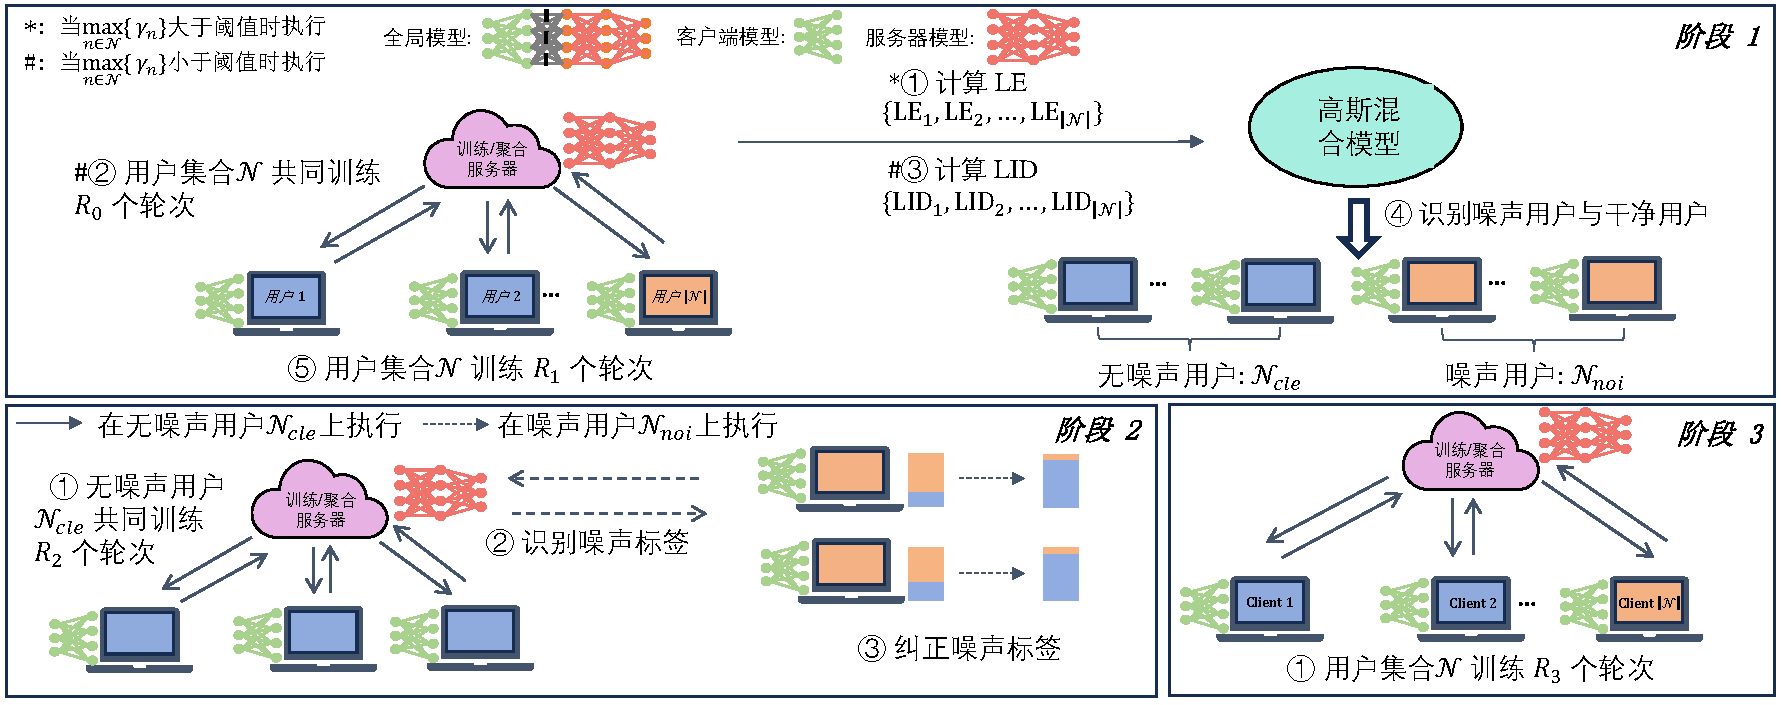
\includegraphics[width=\linewidth]{figures/al.pdf}
\caption{SFL-DCT 概览。}
\label{fig:SFL-DCT}
\end{figure}

\begin{figure}[t]
\centering
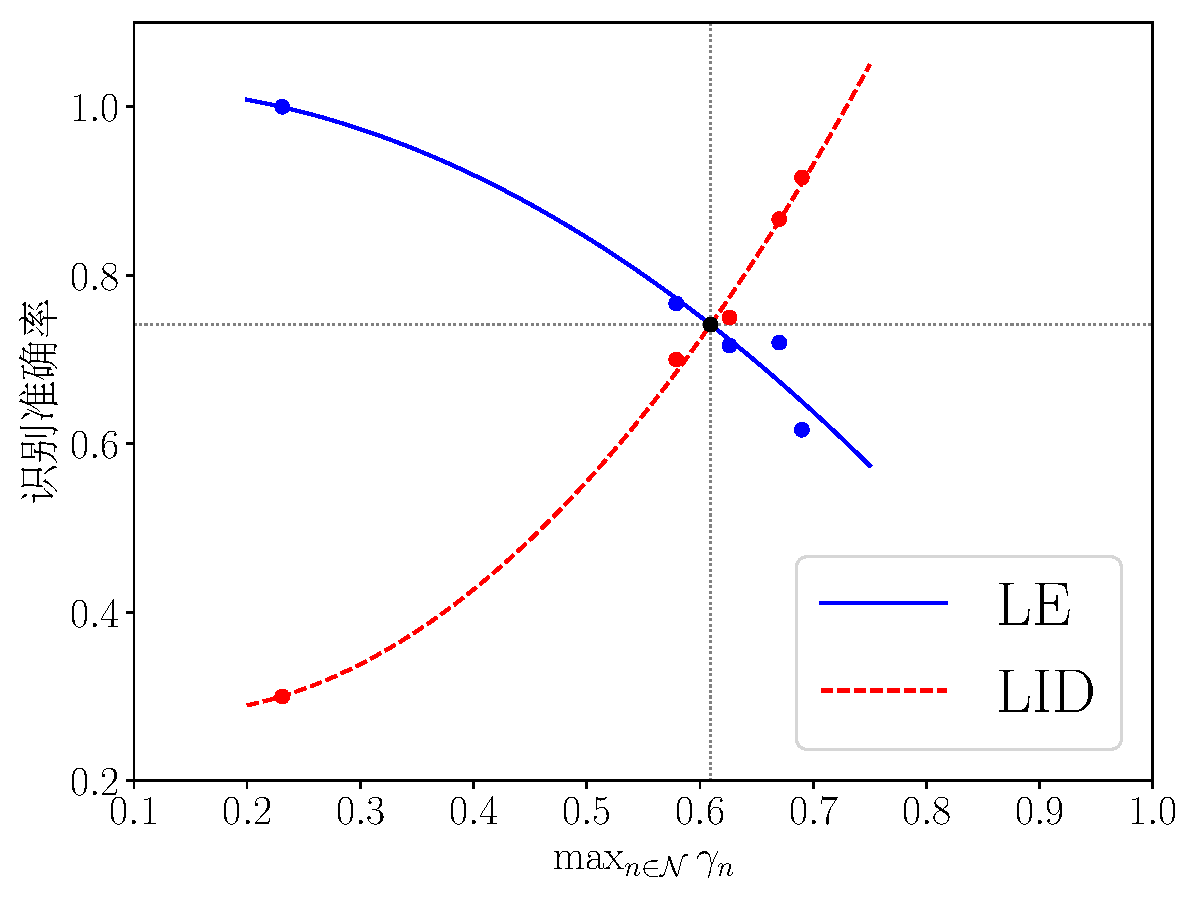
\includegraphics[height=5.3cm]{figures/gamma.pdf}
\caption{通过 LE 和 LID 方法检测含噪用户的准确率与 $\max_{n\in \mathcal{N}} \gamma_n$ 的关系。}
\label{fig:gamma}
\end{figure}

第一阶段的目标是检测存在标签噪声的客户端。在分割-联邦学习中，客户端会在训练过程中将标签发送给服务器 \cite{thapa2022splitfed,huang2023minibatch}。服务器为每个客户端 $n$ 计算一个系数 $\gamma_n$，用以反映该客户端数据集的非独立同分布（non-IID）程度。

为了计算 $\gamma_n$，服务器按升序排列客户端 $n$ 的标签频率。设 $(y_{(1)}^n, y_{(2)}^n, \dots, y_{(|\mathcal{K}|)}^n)$ 表示排序后的标签。

然后，$\gamma_n$ 通过计算前 $\lfloor K/{2}\rfloor$ 个标签所占数据样本的比例来确定：
\begin{equation}\label{calculate dn}
\gamma_n = \frac{\sum_{i=1}^{\lfloor K/{2}\rfloor} \text{count}(y_{(i)}^n)}{|\D_n|},
\end{equation}
其中 $\text{count}(y_{(i)}^n)$ 表示具有标签 $y_{(i)}^n$ 的数据样本数量。

根据所有 $n\in\N$ 的 $\gamma_n$ 值，我们选择合适的方法来检测含噪客户端。有两种候选方法：基于 LID 的检测和基于 LE 的检测。前者来源于文献 \cite{b9}，更适合 IID 数据集场景；后者则更适用于 non-IID 数据集。我们建议使用 $\max_{n\in \mathcal{N}} \gamma_n$ 来判断是否存在数据集极度非 IID 的客户端（即仅包含有限种类的标签）。如果 $\max_{n \in \mathcal{N}} \gamma_n > \tau$，则优先采用基于 LE 的方法；否则推荐使用基于 LID 的方法。其中，$\tau$ 是一个可以通过实验经验确定的阈值。

以 CIFAR-10 数据集为例，图~\ref{fig:gamma} 中的两条曲线展示了在不同 $\max_{n \in \mathcal{N}} \gamma_n$ 值下，LE 和 LID 方法检测含噪客户端的准确率。这两条曲线的交点表示最优的 $\tau$ 值，在该点上两种方法的性能达到平衡。对于这两种方法，训练服务器会通过计算每个客户端的 LID 分数或 LE 分数来评估其是否含有标签噪声。

\textbf{LID 分数：} 为了计算客户端的 LID 分数，首先让客户端使用 SFL 对全局模型进行 $R_0$ 轮训练。根据训练输出，对每个数据点 $(x_i,\tilde{y}_i)$，其 LID 定义如下 \cite{b9,amsaleg2015estimating,houle2013dimensionality}：
\begin{align}\label{eq:lid}
\text{LID}(x_i,\tilde{y}_i)=-\left(\frac{1}{k}\sum_{j=1}^k\log\frac{d_j\left(h\left(x_i,\omegab\right)\right)}{d_{max}\left(h\left(x_i,\omegab\right)\right)}\right)^{-1}.
\end{align}
在式 \eqref{eq:lid} 中，$d_j\left(h\left(x_i,\omegab\right)\right)$ 表示数据样本 $(x_i,\tilde{y}_i)$ 与其邻近样本 $(x_j,\tilde{y}_j)$ 在特征空间中的欧氏距离。考虑 $(x_i,\tilde{y}_i)$ 的 $k$ 个最近邻样本，即 $k$ 个具有最小 $d_j\left(h\left(x_i,\omegab\right)\right)$ 的样本。令 $d_{max}\left(h\left(x_i,\omegab\right)\right)$ 表示在这 $k$ 个最近邻中与 $(x_j,\tilde{y}_j)$ 的最大距离。

直观上讲，定义在 \eqref{eq:lid} 中的数据样本 LID 反映了该样本与其他样本的接近程度，从而间接揭示了其标签可能为噪声标签的可能性。每个客户端 $n$ 的 LID 分数为其数据集 $\mathcal{D}_n$ 中所有样本 LID 值的平均值：
% \begin{figure}[t]
% % \vspace{-15pt}
% \centering
% 
\includegraphics[height=3.3cm]{pic/demo.pdf} 
\includegraphics[height=3.3cm]{pic/time.pdf}\\
% (a)\qquad\qquad\qquad\qquad\qquad\qquad(b)
% % \vspace{-5pt}
% \caption{系统设计（a）与时间流程图（b）演示。}
% \label{fig:demo}
% % \vspace{-10pt}
% \end{figure}
\begin{equation}\label{definition of lid}
\textstyle \text{LID}_n = \sum_{(x_i,\tilde{y}_i)\in\D_{n}} \text{LID}(x_i,\tilde{y}_i)/|\D_n|.
\end{equation}

\textbf{LE 分数：} 我们提出使用标签的熵来衡量标签噪声。这一想法源于一个直观认识：随机噪声会使标签分布变得不那么集中。具体而言，LE 分数的计算方式如下：
\begin{equation}\label{eq:LE}
\text{LE}_n=-\gamma_n\log(\gamma_n)-(1-\gamma_n)\log(1-\gamma_n).
\end{equation}

随后，SFL-DCT 使用高斯混合模型（GMM）对 LID 或 LE 分数进行分类，从而区分干净客户端与含噪客户端。接着，SFL 训练过程继续进行，直到完成 $R_1$ 轮训练。需要注意的是，LID 的计算需要 $R_0$ 轮训练，而 LE 则不需要。进行至 $R_1$ 轮的训练确保了基于 LID 和基于 LE 的方法在相同训练水平上进行比较。

第二阶段通过使用被归类为干净的客户端（即 $n \in \mathcal{N}_{cle}$）来训练全局模型 $\omegab$，以提升模型准确率。训练损失用于识别每个含噪客户端 $n\in\mathcal{N}_{noi}$ 数据集中的噪声标签，因为噪声数据的损失通常较高。训练好的模型 $\omegab$ 随后被用于修正刚刚检测出的噪声标签。

在第三阶段，所有客户端 $n \in \mathcal{N}$ 在已修正第二阶段中检测出的噪声标签的数据集 $\mathcal{D}_n'$ 上继续进行训练，共进行 $R_3$ 轮。最终，获得优化后的全局模型。

\subsection{树莓派测试平台的实现}\label{sec:testbed}
\begin{figure}[t]
\centering
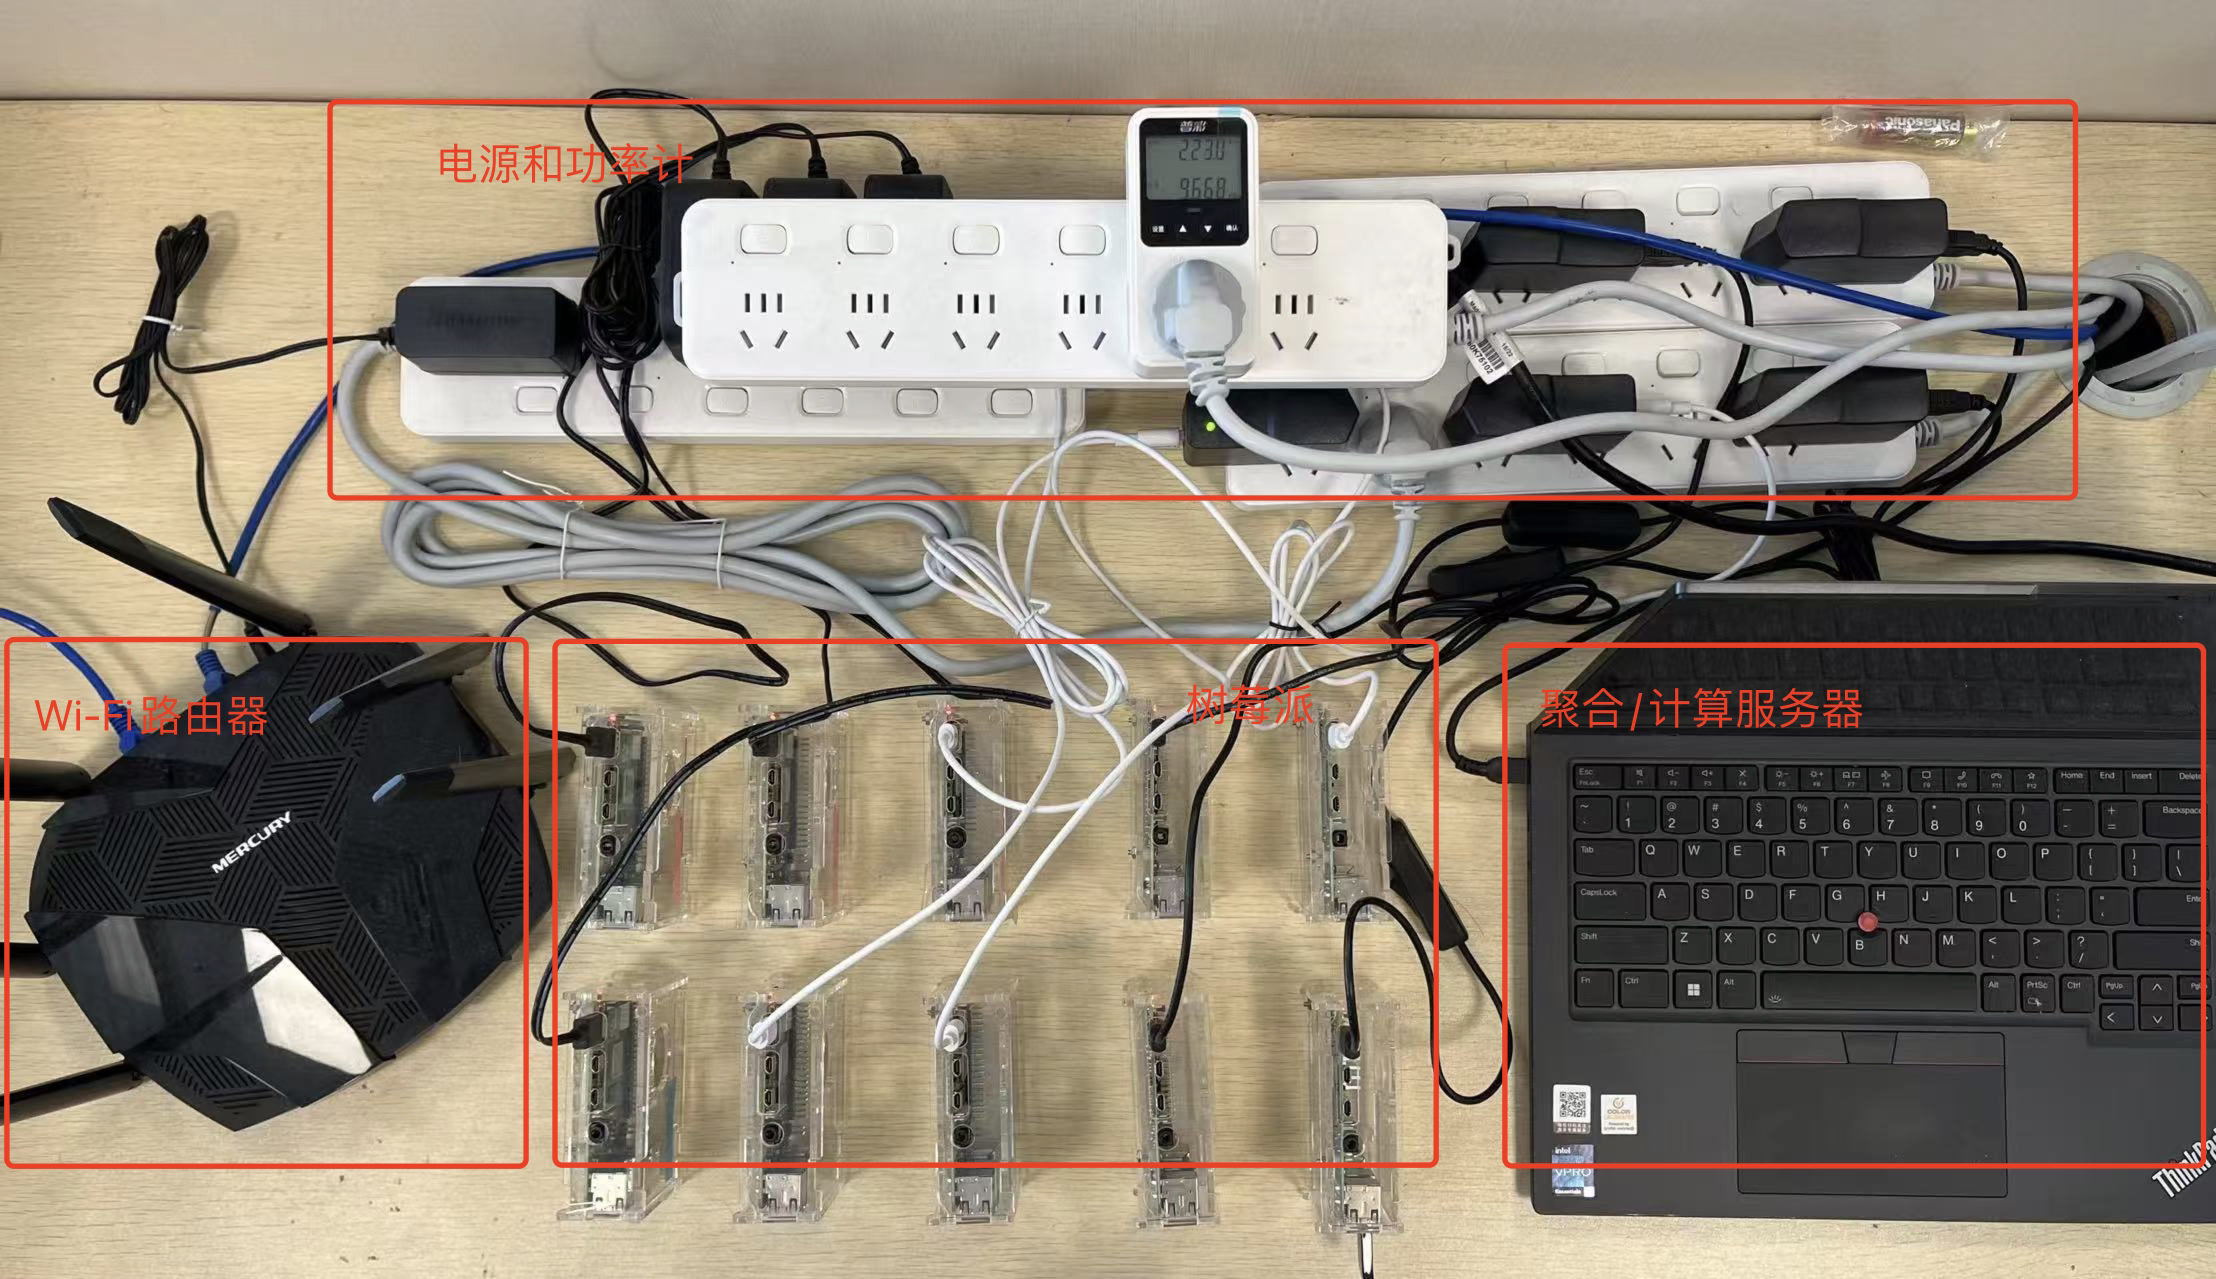
\includegraphics[height=4.5cm]{figures/testbed.png}
% \vspace{-5pt}
\caption{真实测试平台。}
\label{fig:testbed}
% \vspace{-15pt}
\end{figure}
在我们搭建的测试平台上，联邦服务器（fed server）和训练服务器（training server）部署在同一台个人电脑上（处理器为 13th Gen Intel(R) Core(TM) i7-13700K）。10个 Raspberry Pi 4B 设备作为客户端运行。由于 HTTP 协议具有较强的抗无线错误和丢包能力，我们在数据传输（如模型和梯度传输）中采用了 HTTP 协议。

每个客户端包含三个模块：客户端侧训练模块、HTTP 下载模块和客户端 HTTP 代理模块。服务器端则包括联邦服务器模块、训练服务器模块、HTTP 下载器模块以及 $N$ 个服务器端 HTTP 代理模块。HTTP 下载器与代理模块负责协调客户端与服务器之间的数据传输，同时支持并行数据交换（即双工通信，并允许多个客户端同时发送或接收数据）。

为了通过 HTTP 实现数据传输，每次数据传输都由一个 HTTP 请求触发。这种设计确保了数据交换的高效性与准确性，从而降低了分割-联邦学习的训练延迟，因为 HTTP 协议能够保证可靠的数据传输。


\section{实验部分}
\subsection{分割-联邦学习收敛性的实验验证}
\subsubsection{实验设置}
我们在 CIFAR-10 和 CIFAR-100数据集上进行了实验。 两个数据集均包含 6 万张图像（5 万张用于训练，1 万张用于测试），不同之处在于 CIFAR-10 包含 10 个类别，而 CIFAR-100 包含 100 个类别。我们使用交叉熵作为损失函数。

为了模拟数据异构性，我们采用了广泛使用的 Dirichlet 分布 \cite{hsu2019measuring}，并引入一个控制参数 $\alpha$。其中，较小的 $\alpha$ 值表示客户端之间的数据异构性更高。我们选用 ResNet-18 作为模型结构，该网络包含四个残差块，并考虑四种模型切分方式，分别由 $L_c=\{1,2,3,4\}$ 表示，其中 $L_c=n$ 表示模型在第 $n$ 个残差块之后进行切分。

我们将两种主流分布式学习方法作为基准进行比较：联邦学习（FL，特别是 FedAvg \cite{mcmahan2017communication}）和分割学习（SL）\cite{vepakomma2018split}。SFL-V1、SFL-V2、FL 和 SL 的学习率统一设置为 $0.01$。批量大小 $b_s = 128$，实验运行总轮数为 $T=200$ 轮。

我们使用以下参数设置：客户端数量 $N=10$，数据异构性参数 $\beta=0.1$，本地训练轮数 $E=5$，其中 $E$ 表示客户端模型聚合前的本地训练次数（即每对每个客户端的数据进行 $E$ 次训练后，其客户端侧模型将在联邦服务器上进行聚合），因此 $\tau=\lceil \frac{D_n}{b_s}\rceil\times E$。为了与标准联邦学习进行公平比较，我们将 $\tau$ 设置为与 $\tilde{\tau}$ 相等。
所有实验运行在 CPU（Intel(R) Xeon(R) Gold 5320 @ 2.20GHz）和 GPU（A100-PCIE-80GB）平台上。
\subsubsection{实验结果}
在分割-联邦学习中，各类超参数豆会对于模型的收敛产生影响，本部分实验目标是验证分割-联邦学习在不同超参数下的收敛规律。

每轮训练时数据的迭代次数$E$是可以选择的。一般而言，$E$的值过小可能导致用户的模型在没有学习到足够的信息时就
被联邦服务器聚合，学到的信息也随之消散；$E$的值过大可能导致用户的模型在非独立同分布的数据上产生过大的偏差，联邦服务器无法
将大量存在过大偏差的模型聚合为无偏差的模型。本文选择$E \in \{2,5,10\}$三个值进行实验。根据图\ref{fig:multi-image9}显示，模型的最终准确率
相差无几，但$E=2$时模型的收敛速率更快。
\begin{figure}[H]
\centering
\subcaptionbox{SFL-V1\label{fig:subfi}}
{
\includegraphics[width=0.4\linewidth]{E1.pdf}}
\subcaptionbox{SFL-V2\label{fig:sub}}
{
\includegraphics[width=0.4\linewidth]{E2.pdf}}
\caption{每轮训练数据迭代次数E对准确率的影响}
\label{fig:multi-image9}
\end{figure}

参与训练的用户数$N$也会对模型的准确率产生很大的影响。用户数量较少时，每一个用户可以在
全局模型中占有较大的比重，可以提升全局模型在所有用户上的泛化能力。但同时全局模型也可能被不均匀的数据严重
影响，导致准确率低下。用户数量较多时，每一个用户的模型在全局模型中的比重降低，会降低全局模型的泛化能力。但同时，
单个用户的不均匀数据对全局模型的影响也会降低。本文选择$N\in\{10,50,100\}$三个值进行实验。根据图\ref{fig:multi-image00}显示模型的最终准确率差别不大，
$N$越大时模型的收敛速率越慢。
\begin{figure}[H]
\centering
\subcaptionbox{SFL-V1\label{fig:subfin}}
{
\includegraphics[width=0.4\linewidth]{N1.pdf}}
\subcaptionbox{SFL-V2\label{fig:subn}}
{
\includegraphics[width=0.4\linewidth]{N2.pdf}}
\caption{参与训练的用户数$N$对准确率的影响}
\label{fig:multi-image00}
\end{figure}
每轮参与训练的用户比例$q$会显著影响模型的准确率和收敛速率。当每轮参与训练的比例过低时，
模型每轮难以学习到足够的信息，且模型获得的信息总是带有偏向性的，这种情况会严重影响模型的训练。本文选择$q\in\{0.2,0.5,1\}$
三个值进行实验。根据图\ref{fig:multi-image0000}显示，随着q的增大，模型的收敛速率加快的同时，最终准确率也会提高。
\begin{figure}[H]
\centering
\subcaptionbox{SFL-V1\label{fig:subfiq}}
{
\includegraphics[width=0.4\linewidth]{q1.pdf}}
\subcaptionbox{SFL-V2\label{fig:subq}}
{
\includegraphics[width=0.4\linewidth]{q2.pdf}}
\caption{每轮参与训练的用户比例$q$对准确率的影响}
\label{fig:multi-image0000}
\end{figure}

\subsection{分割-联邦学习鲁棒性算法的实验验证}

\subsubsection{实验设置}
客户端数据同样采用Dirichlet分布进行采样，并且也引入控制参数 $\alpha$\cite{hsu2019measuring}。其中，$\alpha$ 的值越大，表示数据异构性越低。我们考虑两种场景：独立同分布（IID，$\alpha=\infty$）和非独立同分布（non-IID，$\alpha=0.1$）。与 \cite{b9,ji2024fedfixer,li2024feddiv} 类似，我们通过随机翻转标签的方式模拟标签噪声，即以一定概率（称为噪声率）将样本的标签随机翻转为其他类别。我们在 CIFAR-10 和 CIFAR-100 数据集上设置了 $\{0, 10\%, 20\%, 30\%, 40\%, 50\%, 60\%\}$ 的噪声率，在 Fashion-MNIST 上设置了 $\{40\%, 50\%, 60\%, 70\%, 80\%\}$ 的噪声率。为了便于观察实验结果，我们仅展示了部分噪声设置下的实验结果。

用于训练 SFL 模型的数据集、模型结构以及客户端数量如表 \ref{table:hyper-parameters} 所示。
主要的超参数如下：批量大小设为 128；学习率为 $\eta^r=0.01$；每轮训练使用 $E=5$ 个 epoch。
我们使用交叉熵作为损失函数。实验所用 GPU 为 A100-80GB，每次训练仅使用一块 GPU。
\begin{table}[t]
\caption{不同数据集的设置}
\begin{center}
\begin{tabular}{cccc}
\hline
数据集 & CIFAR-10 & CIFAR-100 & Fashion-MNIST \\ \hline
客户端数量 & 100 & 100 & 50 \\ 
模型 & ResNet-18 & ResNet-34 & 10层CNN \\ \hline
\end{tabular}
\label{table:hyper-parameters}
\end{center}
\end{table}
\subsection{SFL-DCT的结果}

我们现在评估所提出算法 SFL-DCT 的性能。我们假设在此场景下有 60\% 的客户端存在标签噪声\cite{b9,ji2024fedfixer,li2024feddiv}。我们将 SFL-DCT 与两种现有的去噪算法（FedCorr\cite{b9} 和 FedNoRo\cite{wu2023fednoro}）以及两种基线算法（SFL-V2 和 SFL-V1/FL）\footnote{由于 SFL-V1 与 FedAvg 在逻辑上是相同的算法，因此 SFL-V1 的结果也可以代表 FedAvg。}\cite{thapa2022splitfed} 进行了比较。为了公平比较，我们将这些现有去噪算法转换为基于分割-联邦学习的形式。具体来说，模型被划分为客户端和服务器两部分，训练过程遵循图~\ref{fig:sfl} 中所示的步骤 1 - 步骤 4。在模型聚合阶段，仅对客户端侧模型进行联邦更新，如图~\ref{fig:sfl} 中步骤 5 所示。


表 \ref{table:compare cifar10}、\ref{table:compare cifar100} 和 \ref{table:compare fmnist} 分别展示了不同算法在 CIFAR-10、CIFAR-100 和 Fashion-MNIST 数据集上的平均最佳准确率（3 次实验取平均）。我们观察到，不论用户间的数据是否独立同分布，标签噪声对 SFL-DCT 的影响均小于基线算法（即 SFL-V2 和 SFL-V1/FL）。这是因为 SFL-DCT 能够有效检测并纠正标签，从而显著减轻由标签噪声带来的性能下降。与这两种去噪算法（FedCorr 和 FedNoRo）相比，SFL-DCT 在各种设置下均展现出更优的性能。在数据独立同分布场景下，大多数情况下 SFL-DCT 的准确率略高于这两个竞争算法；而在数据非独立同分布场景下，其表现明显优于它们，体现出更强的鲁棒性和更高的准确性。
\begin{table*}[t]
\caption{CIFAR-10 数据集上各算法的最佳平均准确率}
\begin{center}
\resizebox{\textwidth}{!}{
\begin{tabular}{c|cccccccccccc}
\hline\hline
\multicolumn{1}{c|}{\multirow{3}{*}{算法}} & \multicolumn{12}{c}{测试准确率(\%)} \\ \cline{2-13} 
\multicolumn{1}{c|}{} & \multicolumn{6}{c|}{IID} & \multicolumn{6}{c}{Non-IID} \\ \cline{2-13} 
\multicolumn{1}{c|}{} & \multicolumn{1}{c|}{$\delta$ = 0.1} & \multicolumn{1}{c|}{$\delta$ = 0.2} & \multicolumn{1}{c|}{$\delta$ = 0.3} & \multicolumn{1}{c|}{$\delta$ = 0.4} & \multicolumn{1}{c|}{$\delta$ = 0.5} & \multicolumn{1}{c|}{$\delta$ = 0.6} & \multicolumn{1}{c|}{$\delta$ = 0.1} & \multicolumn{1}{c|}{$\delta$ = 0.2} & \multicolumn{1}{c|}{$\delta$ = 0.3} & \multicolumn{1}{c|}{$\delta$ = 0.4} & \multicolumn{1}{c|}{$\delta$ = 0.5} & \multicolumn{1}{c}{$\delta$ = 0.6} \\ \hline
SFL-DCT & \multicolumn{1}{c}{84.66} & \multicolumn{1}{c}{\textbf{83.84}} & \multicolumn{1}{c}{\textbf{83.15}} & \multicolumn{1}{c}{\textbf{83.15}} & \multicolumn{1}{c}{\textbf{83.07}} & \multicolumn{1}{c}{\textbf{82.07}} & \multicolumn{1}{c}{\textbf{67.20}} & \multicolumn{1}{c}{\textbf{68.31}} & \multicolumn{1}{c}{\textbf{66.15}} & \multicolumn{1}{c}{\textbf{63.12}} & \multicolumn{1}{c}{\textbf{63.33}} & \multicolumn{1}{c}{\textbf{60.99}} \\ 
SFL-V1 & \multicolumn{1}{c}{84.26} & \multicolumn{1}{c}{78.29} & \multicolumn{1}{c}{75.50} & \multicolumn{1}{c}{70.84} & \multicolumn{1}{c}{66.01} & \multicolumn{1}{c}{63.35} & \multicolumn{1}{c}{62.18} & \multicolumn{1}{c}{56.30} & \multicolumn{1}{c}{50.97} & \multicolumn{1}{c}{45.13} & \multicolumn{1}{c}{41.62} & \multicolumn{1}{c}{38.75} \\ 
SFL-V2 & \multicolumn{1}{c}{84.33} & \multicolumn{1}{c}{78.90} & \multicolumn{1}{c}{74.99} & \multicolumn{1}{c}{70.92} & \multicolumn{1}{c}{67.57} & \multicolumn{1}{c}{64.83} & \multicolumn{1}{c}{65.72} & \multicolumn{1}{c}{59.13} & \multicolumn{1}{c}{53.31} & \multicolumn{1}{c}{47.43} & \multicolumn{1}{c}{43.78} & \multicolumn{1}{c}{40.98} \\ 
FedCorr & \multicolumn{1}{c}{\textbf{84.95}} & \multicolumn{1}{c}{83.11} & \multicolumn{1}{c}{82.90} & \multicolumn{1}{c}{82.63} & \multicolumn{1}{c}{82.11} & \multicolumn{1}{c}{81.46} & \multicolumn{1}{c}{63.71} & \multicolumn{1}{c}{57.36} & \multicolumn{1}{c}{51.10} & \multicolumn{1}{c}{46.92} & \multicolumn{1}{c}{41.60} & \multicolumn{1}{c}{39.68} \\ 
FedNoRo & \multicolumn{1}{c}{84.37} & \multicolumn{1}{c}{81.71} & \multicolumn{1}{c}{81.02} & \multicolumn{1}{c}{79.35} & \multicolumn{1}{c}{77.58} & \multicolumn{1}{c}{76.14} & \multicolumn{1}{c}{58.43} & \multicolumn{1}{c}{54.19} & \multicolumn{1}{c}{52.74} & \multicolumn{1}{c}{48.90} & \multicolumn{1}{c}{44.54} & \multicolumn{1}{c}{40.76} \\ \hline
\end{tabular}
}
\label{table:compare cifar10}
\end{center}
\end{table*}
\begin{table*}[t]
\caption{Fashion-MNIST 数据集上各算法的测试准确率}
\begin{center}
\resizebox{\textwidth}{!}{
\begin{tabular}{l|llllllllll}
\hline\hline
\multicolumn{1}{c|}{\multirow{3}{*}{算法}} & \multicolumn{10}{c}{测试准确率(\%)} \\ \cline{2-11} 
\multicolumn{1}{c|}{} & \multicolumn{5}{c|}{IID} & \multicolumn{5}{c}{Non-IID} \\ \cline{2-11} 
\multicolumn{1}{c|}{} & \multicolumn{1}{c|}{$\delta$ = 0.4} & \multicolumn{1}{c|}{$\delta$ = 0.5} & \multicolumn{1}{c|}{$\delta$ = 0.6} & \multicolumn{1}{c|}{$\delta$ = 0.7} & \multicolumn{1}{c|}{$\delta$ = 0.8} & \multicolumn{1}{c|}{$\delta$ = 0.4} & \multicolumn{1}{c|}{$\delta$ = 0.5} & \multicolumn{1}{c|}{$\delta$ = 0.6} & \multicolumn{1}{c|}{$\delta$ = 0.7} & \multicolumn{1}{c}{$\delta$ = 0.8} \\ \hline
SFL-DCT & \multicolumn{1}{c}{\textbf{89.31}} & \multicolumn{1}{c}{\textbf{89.42}} & \multicolumn{1}{c}{\textbf{88.95}} & \multicolumn{1}{c}{\textbf{88.81}} & \multicolumn{1}{c}{\textbf{87.94}} & \multicolumn{1}{c}{\textbf{84.47}} & \multicolumn{1}{c}{\textbf{83.68}} & \multicolumn{1}{c}{\textbf{84.67}} & \multicolumn{1}{c}{\textbf{79.80}} & \multicolumn{1}{c}{\textbf{80.22}} \\ 
SFL-V1 & \multicolumn{1}{c}{85.12} & \multicolumn{1}{c}{84.63} & \multicolumn{1}{c}{84.55} & \multicolumn{1}{c}{83.71} & \multicolumn{1}{c}{83.68} & \multicolumn{1}{c}{74.82} & \multicolumn{1}{c}{71.61} & \multicolumn{1}{c}{66.43} & \multicolumn{1}{c}{64.26} & \multicolumn{1}{c}{64.07} \\ 
SFL-V2 & \multicolumn{1}{c}{86.07} & \multicolumn{1}{c}{85.78} & \multicolumn{1}{c}{85.14} & \multicolumn{1}{c}{84.05} & \multicolumn{1}{c}{83.84} & \multicolumn{1}{c}{75.78} & \multicolumn{1}{c}{72.68} & \multicolumn{1}{c}{66.86} & \multicolumn{1}{c}{65.51} & \multicolumn{1}{c}{66.15} \\ 
FedCorr & \multicolumn{1}{c}{87.72} & \multicolumn{1}{c}{87.64} & \multicolumn{1}{c}{87.13} & \multicolumn{1}{c}{87.20} & \multicolumn{1}{c}{86.83} & \multicolumn{1}{c}{80.24} & \multicolumn{1}{c}{79.31} & \multicolumn{1}{c}{76.63} & \multicolumn{1}{c}{76.35} & \multicolumn{1}{c}{75.23} \\ 
FedNoRo & \multicolumn{1}{c}{86.10} & \multicolumn{1}{c}{85.93} & \multicolumn{1}{c}{84.69} & \multicolumn{1}{c}{84.82} & \multicolumn{1}{c}{83.43} & \multicolumn{1}{c}{81.52} & \multicolumn{1}{c}{80.33} & \multicolumn{1}{c}{80.51} & \multicolumn{1}{c}{78.81} & \multicolumn{1}{c}{78.04} \\ \hline
\end{tabular}
}
\label{table:compare fmnist}
\end{center}
\end{table*}

\begin{table}[t]
\caption{CIFAR-100 数据集（Non-IID 设置）下各算法的最佳平均准确率}
\begin{center}
\resizebox{0.6\textwidth}{!}{
\begin{tabular}{l|llllll}
\hline\hline
\multicolumn{1}{c|}{\multirow{3}{*}{算法}} & \multicolumn{6}{c}{测试准确率(\%)} \\ \cline{2-7} 
\multicolumn{1}{c|}{} & \multicolumn{1}{c|}{$\delta$ = 0.1} & \multicolumn{1}{c|}{$\delta$ = 0.2} & \multicolumn{1}{c|}{$\delta$ = 0.3} & \multicolumn{1}{c|}{$\delta$ = 0.4} & \multicolumn{1}{c|}{$\delta$ = 0.5} & \multicolumn{1}{c}{$\delta$ = 0.6} \\ \hline
SFL-DCT & \multicolumn{1}{c}{\textbf{63.56}} & \multicolumn{1}{c}{\textbf{60.03}} & \multicolumn{1}{c}{\textbf{57.76}} & \multicolumn{1}{c}{\textbf{54.11}} & \multicolumn{1}{c}{\textbf{50.86}} & \multicolumn{1}{c}{\textbf{49.23}} \\ 
SFL-V1 & \multicolumn{1}{c}{60.54} & \multicolumn{1}{c}{54.10} & \multicolumn{1}{c}{46.82} & \multicolumn{1}{c}{43.77} & \multicolumn{1}{c}{40.10} & \multicolumn{1}{c}{35.18} \\ 
SFL-V2 & \multicolumn{1}{c}{61.14} & \multicolumn{1}{c}{54.78} & \multicolumn{1}{c}{47.58} & \multicolumn{1}{c}{43.82} & \multicolumn{1}{c}{39.50} & \multicolumn{1}{c}{35.46} \\ 
FedCorr & \multicolumn{1}{c}{59.49} & \multicolumn{1}{c}{55.55} & \multicolumn{1}{c}{52.16} & \multicolumn{1}{c}{49.15} & \multicolumn{1}{c}{57.37} & \multicolumn{1}{c}{45.62} \\ 
FedNoRo & \multicolumn{1}{c}{58.26} & \multicolumn{1}{c}{56.31} & \multicolumn{1}{c}{52.88} & \multicolumn{1}{c}{50.43} & \multicolumn{1}{c}{55.91} & \multicolumn{1}{c}{48.10} \\ \hline
\end{tabular}
}
\label{table:compare cifar100}
\end{center}
\end{table}

\begin{figure}[t]
\centering
\begin{subfigure}{0.45\linewidth}
\centering
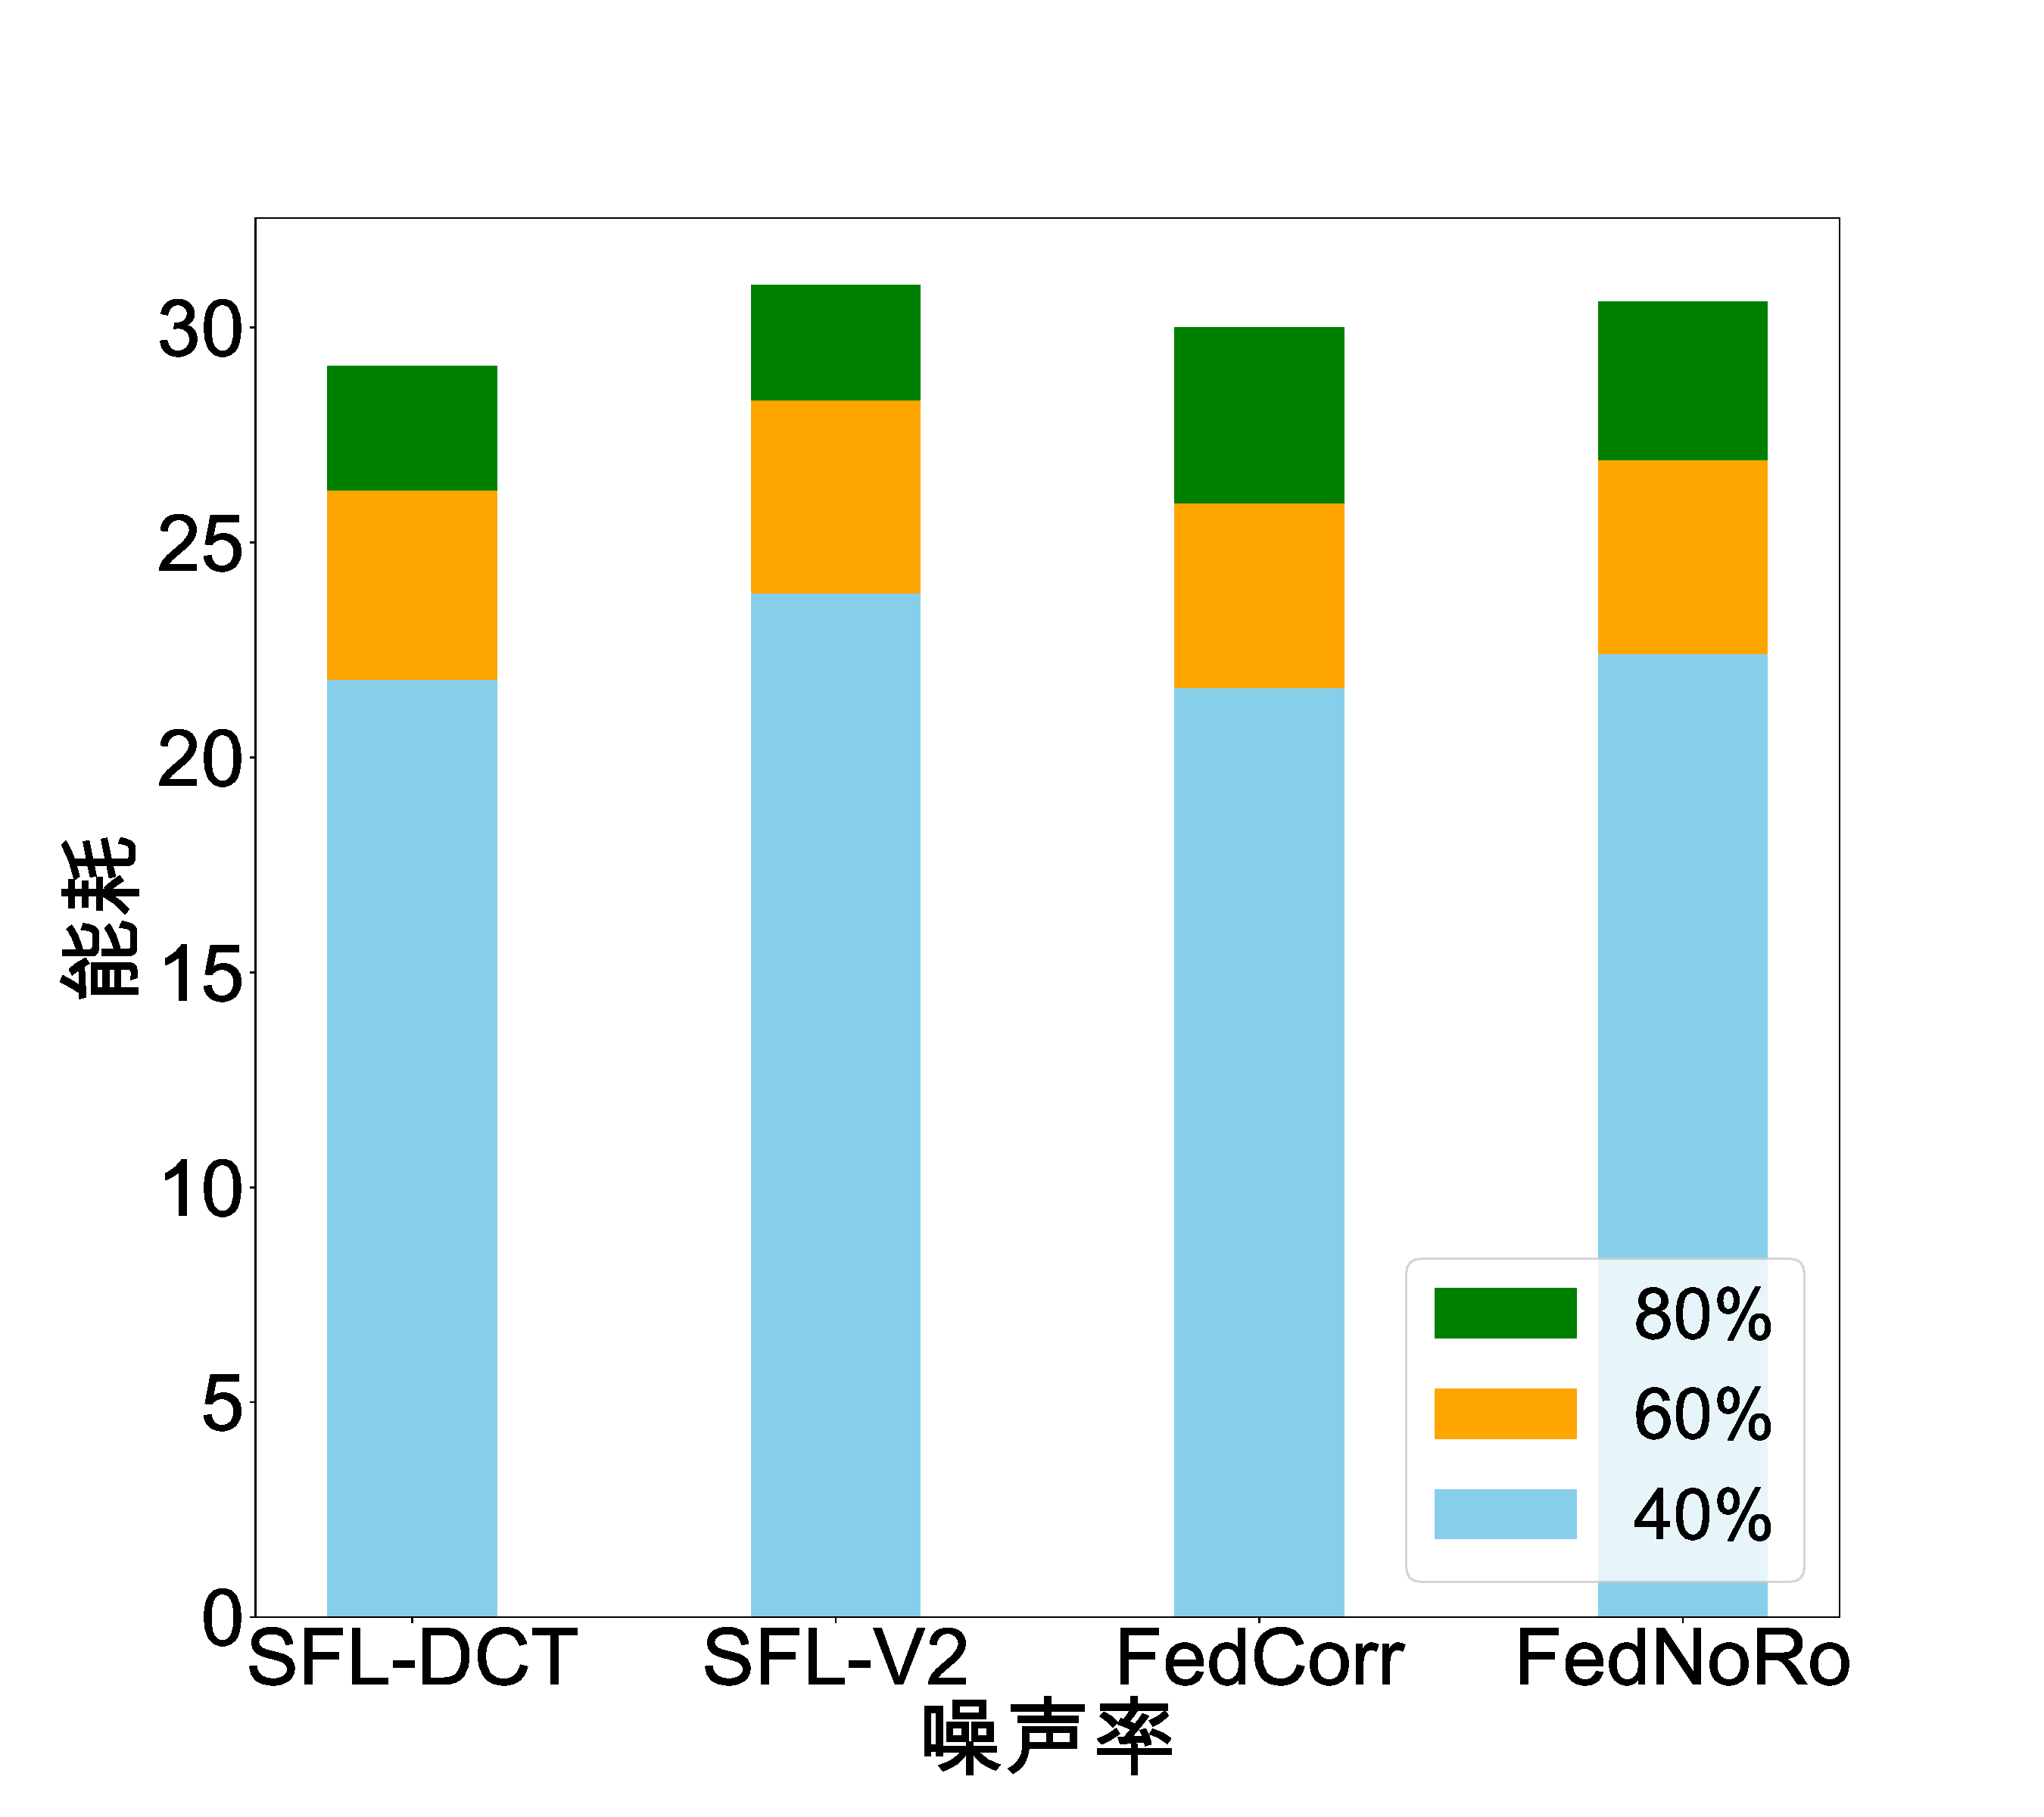
\includegraphics[width=\linewidth]{figures/power_iid.pdf}
\caption{Fashion-MNIST(IID)}
\label{fig:mnist_iid}
\end{subfigure}
\hfill
\begin{subfigure}{0.45\linewidth}
\centering
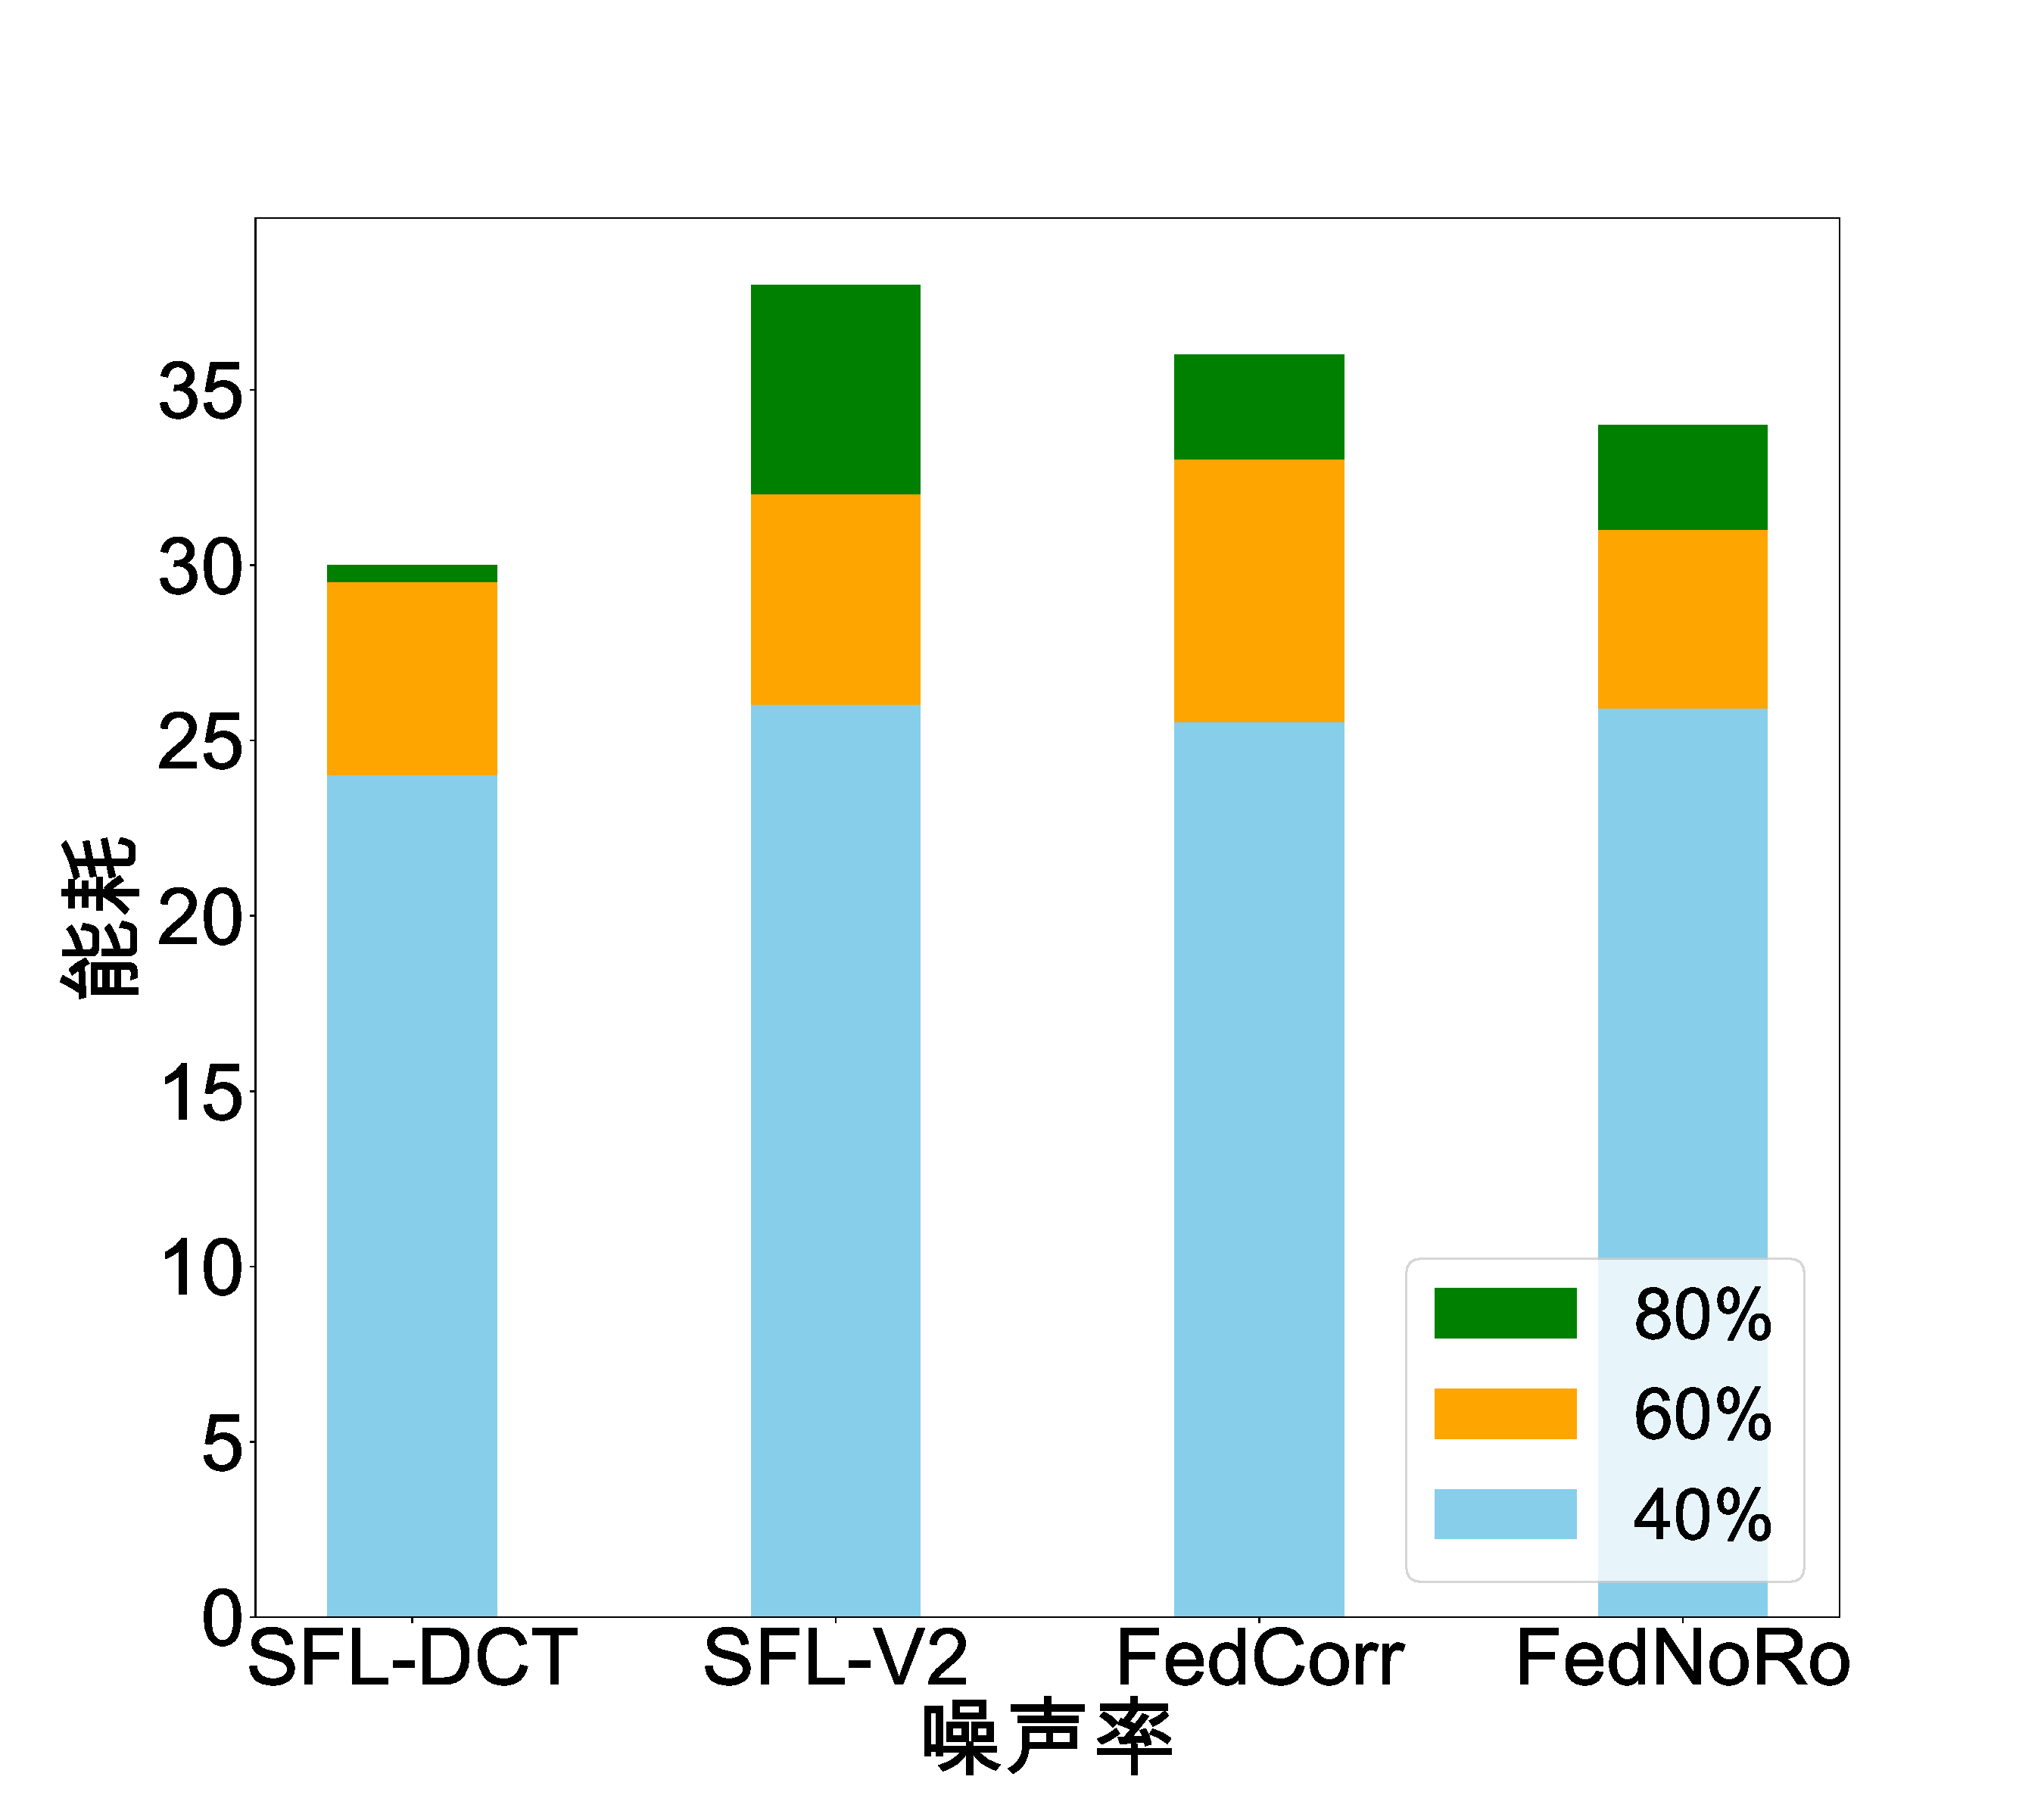
\includegraphics[width=\linewidth]{figures/power_noniid.pdf}
\caption{Fashion-MNIST(non-IID)}
\label{fig:mnist_noniid}
\end{subfigure}
\caption{不同算法的能量消耗对比。}
\label{fig:mnist_energy}
\end{figure}

\subsubsection{SFL-DCT在测试平台上的能耗结果}



我们进一步在测试平台中评估了 SFL-DCT 和 SFL-V2 的实际收敛性和能耗（见第 \ref{sec:testbed} 节）。图 \ref{fig:testbed} 展示了我们的测试平台实验环境。在 SFL-DCT 中，我们将 $R_0$、$R_1$ 和 $R_2$ 设置得远小于 $R_3$，以使得对噪声标签的检测与纠正不会带来显著的计算开销。在每种设置下，我们测量了客户端直到 SFL-V2 收敛时所消耗的能量（单位为 kWh），以便进行公平比较，因为在收敛时 SFL-DCT 的准确率明显高于 SFL-V2。在这个系统中，一个 Raspberry Pi 代表一个客户端，而 PC 作为服务器，它们通过 WIFI 进行通信。我们选用 Fashion-MNIST 数据集，因为它适合计算能力受限的设备。如图 \ref{fig:mnist_energy} 所示，与 SFL-V2 相比，SFL-DCT 在客户端侧显著降低了能耗。在非独立同分布（non-IID）数据下，能耗降低最多可达 23.30\%。



